%\begin{abstract}
%		物理でLegendre変換は解析力学のLagrangianとHamiltonianの関係や熱力学関数たちの関係として与えられる.
%		物理では言及なしにある程度連続微分可能性を仮定するが,
%		熱力学で相転移を扱うときは熱力学関数の微分微分不可能性が効いてくる.
%		多くの教科書では$f^{*}(\alpha) = f(x(\alpha)) - \alpha x(\alpha)$と
%		微分を用いた定義をするが,相転移点も含めた熱力学を議論するとき,$\max$, $\min$
%		\footnote{厳密には$\sup$, $\inf$で与えるが,存在は保証されるそうである\url{https://mathlog.info/articles/829}.}で与える必要がある\cite[付録H]{Tasaki_thermo}, \cite[Chap.11]{thermo_shimizu}.
%\end{abstract}
\subsection{Legendre変換について}
導出として,凸関数$f$に対して,傾き$\alpha$の線を引いたとき,$f$との交点を
持った状態で直線の切片を最小にすることを考える.
$x =x^{*}$を通る直線を引くとき,直線の方程式は
\begin{align}
		y = \alpha x + f(x^{*}) - \alpha x^{*} 
\end{align}
となり,各$\alpha$に対し,切片の最小値を対応させることを考えると次の定義に至る.
\begin{defn}[Legendre変換]
		凸関数$f\colon\R\to\R$に対し,このLegendre変換$f^{*}$を
		\begin{align}
				f^{*}(\alpha) &= -\min_{x\in\R}\qty(f(x)-\alpha x)\\
				 &= \max_{x\in\R}\qty(\alpha x - f(x))\label{def_legendre}
		\end{align}
		と定める.
\end{defn}
このとき,素直に考えると負符号はつかないように思うが,
凸関数を凸関数に移す対称性を持たせるためにはこれが必要である.
\begin{eg}
		関数
		\begin{align}
				f(x)=
				\begin{dcases}
						\frac{x^3+x}{4} ,& (0\leq x \leq 1)\\
						x-\frac{1}{2} ,& (1 \leq x \leq 2)\\
						\frac{x^2}{2} - x + \frac{3}{2} ,& (2\leq x)
				\end{dcases}
		\end{align}
		のLegendre変換は
		\begin{align}
				f^{*}(p) = 
				\begin{dcases}
						\frac{1}{2}\qty(\frac{4p-1}{3})^{3/2} ,& (1/4 < p < 1)\\
						\frac{1}{2}\qty(p^2 + 2p - 2) ,& (1\leq p)
				\end{dcases}
		\end{align}
		となる.

		\footnote{この例は\url{https://ja.wikipedia.org/wiki/\%E3\%83\%AB\%E3\%82\%B8\%E3\%83\%A3\%E3\%83\%B3\%E3\%83\%89\%E3\%83\%AB\%E5\%A4\%89\%E6\%8F\%9B}による.}
\end{eg}
	\begin{figure}[tb]
		\centering
		\begin{minipage}{0.45\linewidth}
				\centering
				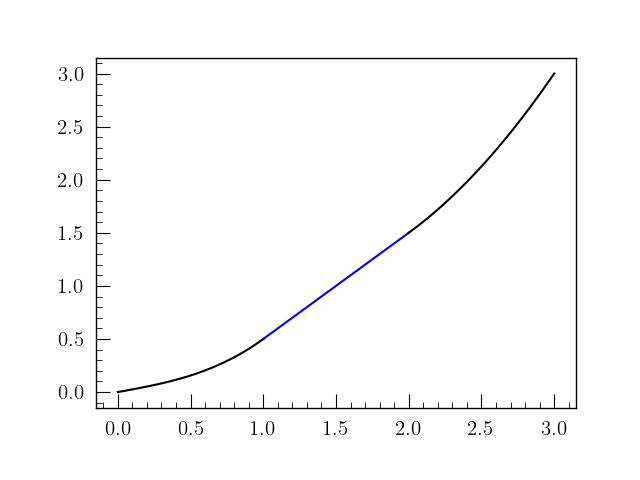
\includegraphics[width=7cm]{./doc/img/eg1_legendre.png}
				\caption{Legendre変換前の関数$f$.}
				\label{fig:before_legendre}
		\end{minipage}
		\begin{minipage}{0.45\linewidth}
				\centering
				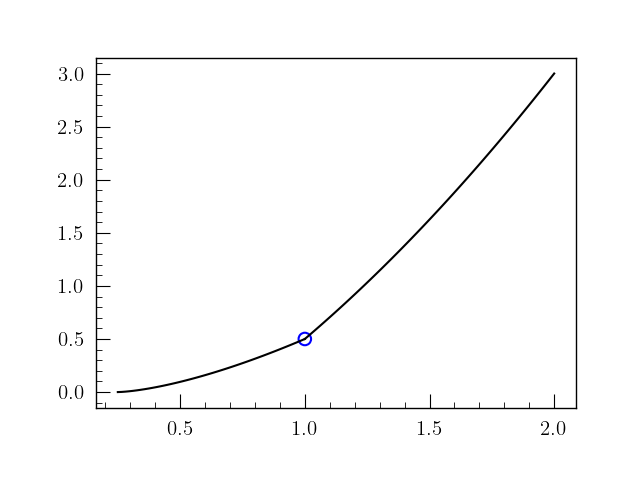
\includegraphics[width=7cm]{./doc/img/eg2_legendre.png}
				\caption{$f$をLegendre変換した関数$f^{*}$}
				\label{fig:after_legendre}
		\end{minipage}

Figure. \ref{fig:before_legendre}の青い線部分が,
Figure. \ref{fig:after_legendre}の一点に潰れていて,微分不可能点になっている.
熱力学関数にこのようなことが起こるとき,相転移が起こっていることがわかる.
\end{figure}
